\section{Problem}\label{sec:problemdef}

In our setting we assume users own an internet enabled mobile device with positioning capabilities. Users issue \spath queries to an online service provider. Users want their \spath result available to them at a speed comparable to that of an offline application.

The \spath service provider want to provide a fast service to its users. The service provider additionally want to save cost on hardware such as CPU and HDD space. The \spath provider therefor wants to return as many \spath results as possible, using the least amount of computation and space.

Using a \spath buffer at the \spath service provider can reduce the CPU cycles used in order to return a \spath result. Doing so would at the same time also increase the responce time of the \spath service, as saving CPU cycles not only allows for more \spaths to be computed on the same hardware, but also allows for returning a buffered result much faster than it would be possible if the \spath had to be found first.

\section{Architecture}
We propose a system where a \spath buffer is implemented in front of an existing \spath service (See fig. \ref{routequery}) such that if the buffer can answer a query then the result can be returned immidiately.

\begin{figure}
  \center
        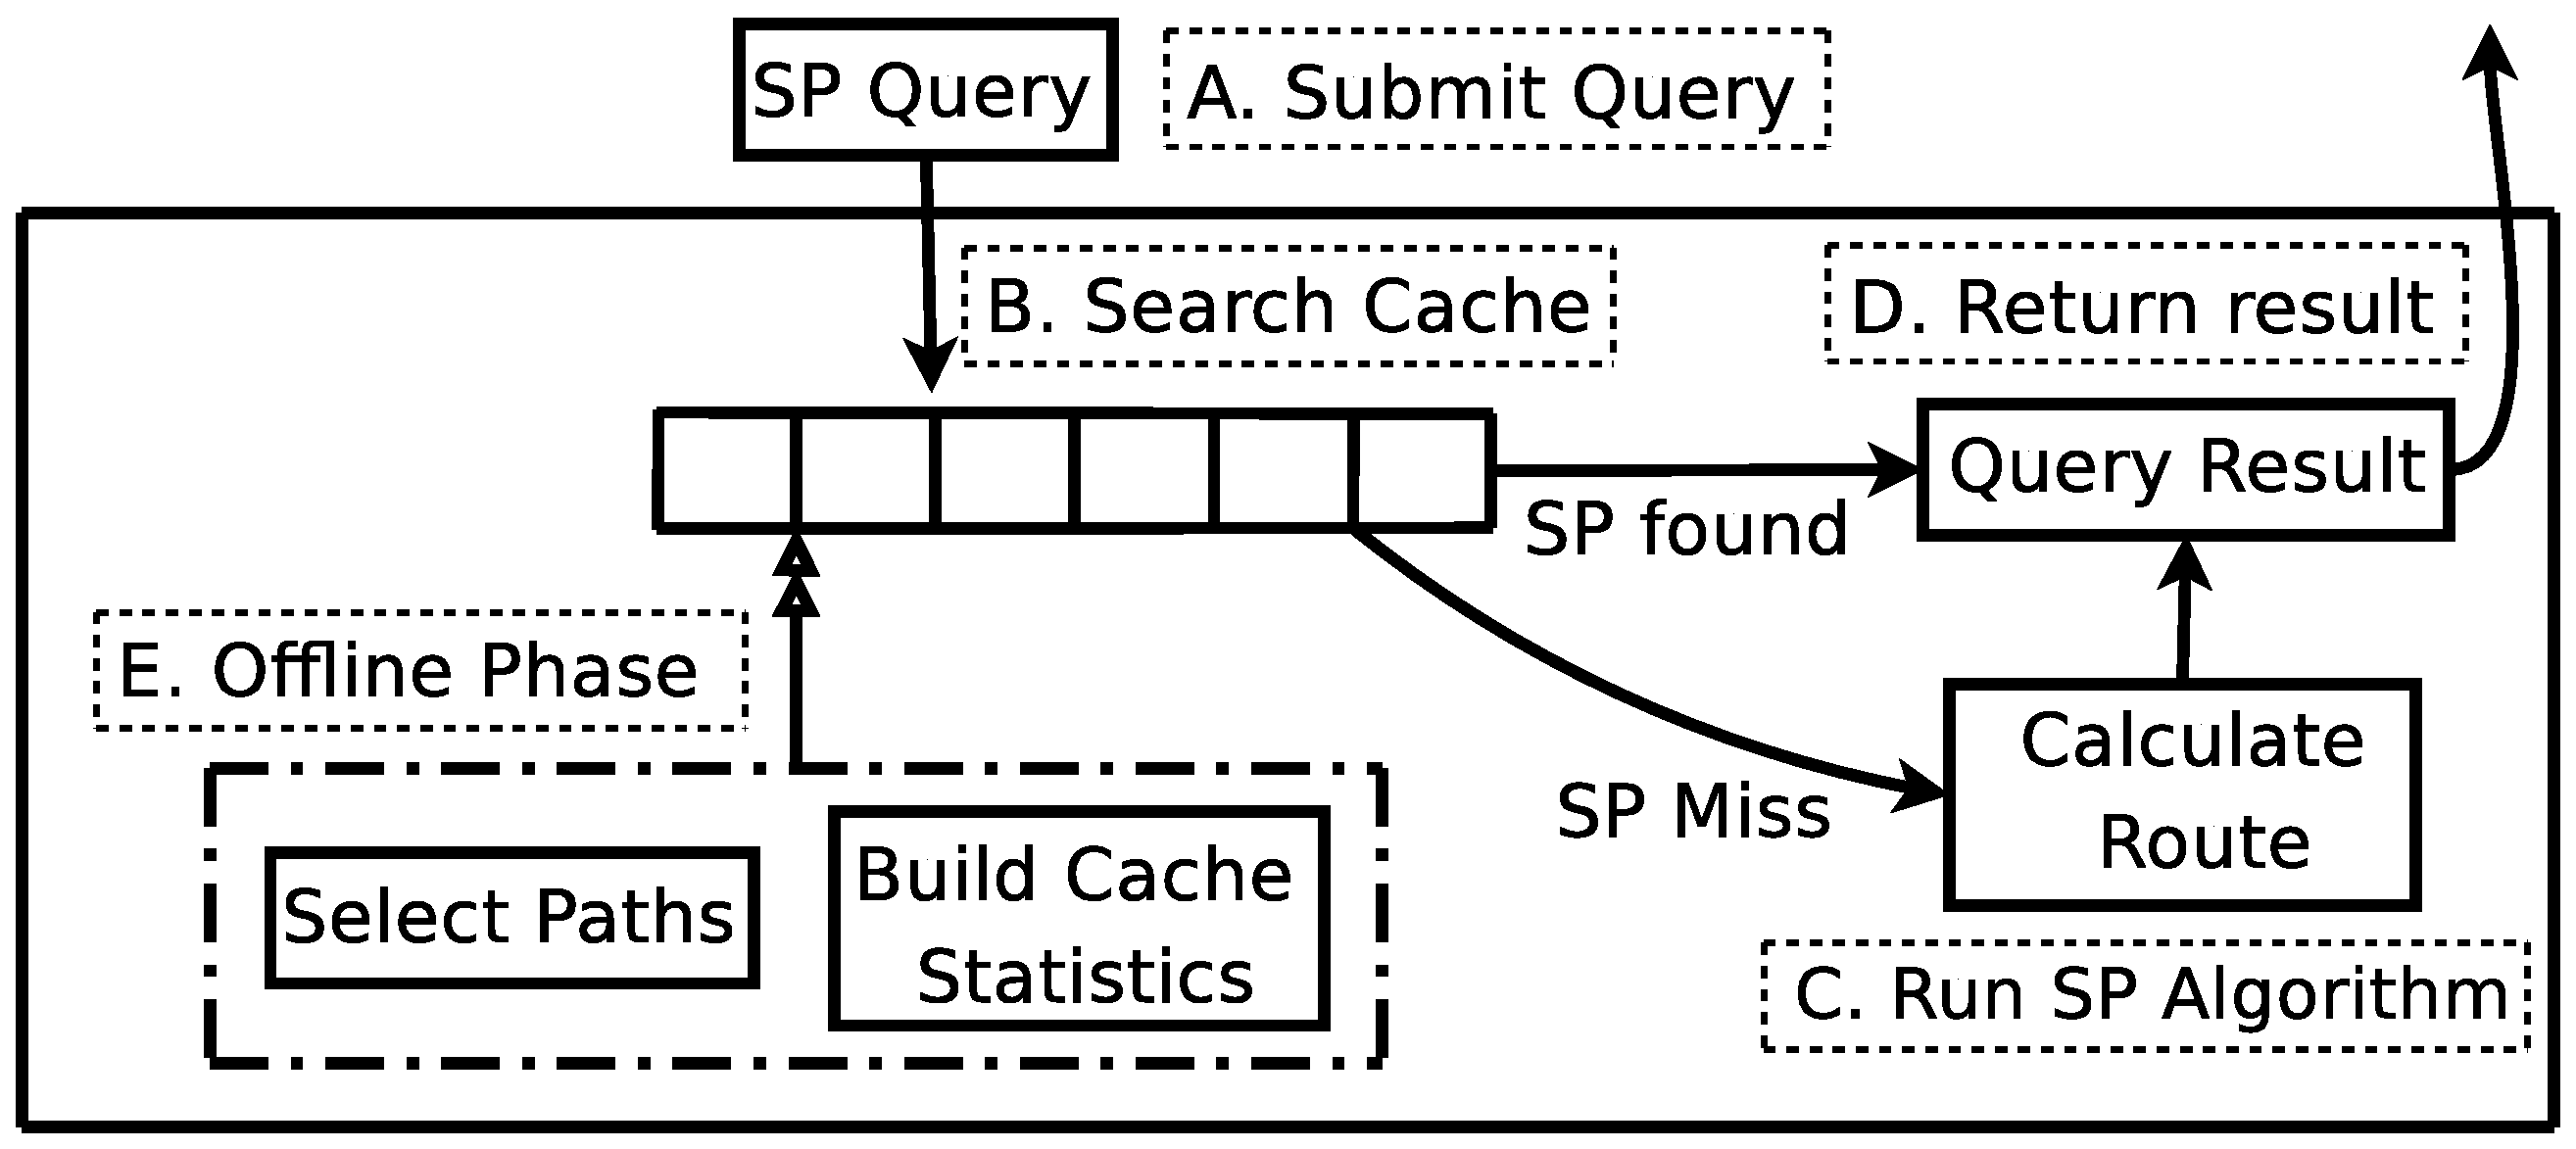
\includegraphics[width=0.5\textwidth]{figures/routequery}
        \caption{Buffer placement in \spath service providers system.}
  \label{fig:routequery}
\end{figure}

\begin{figure}
  \center
        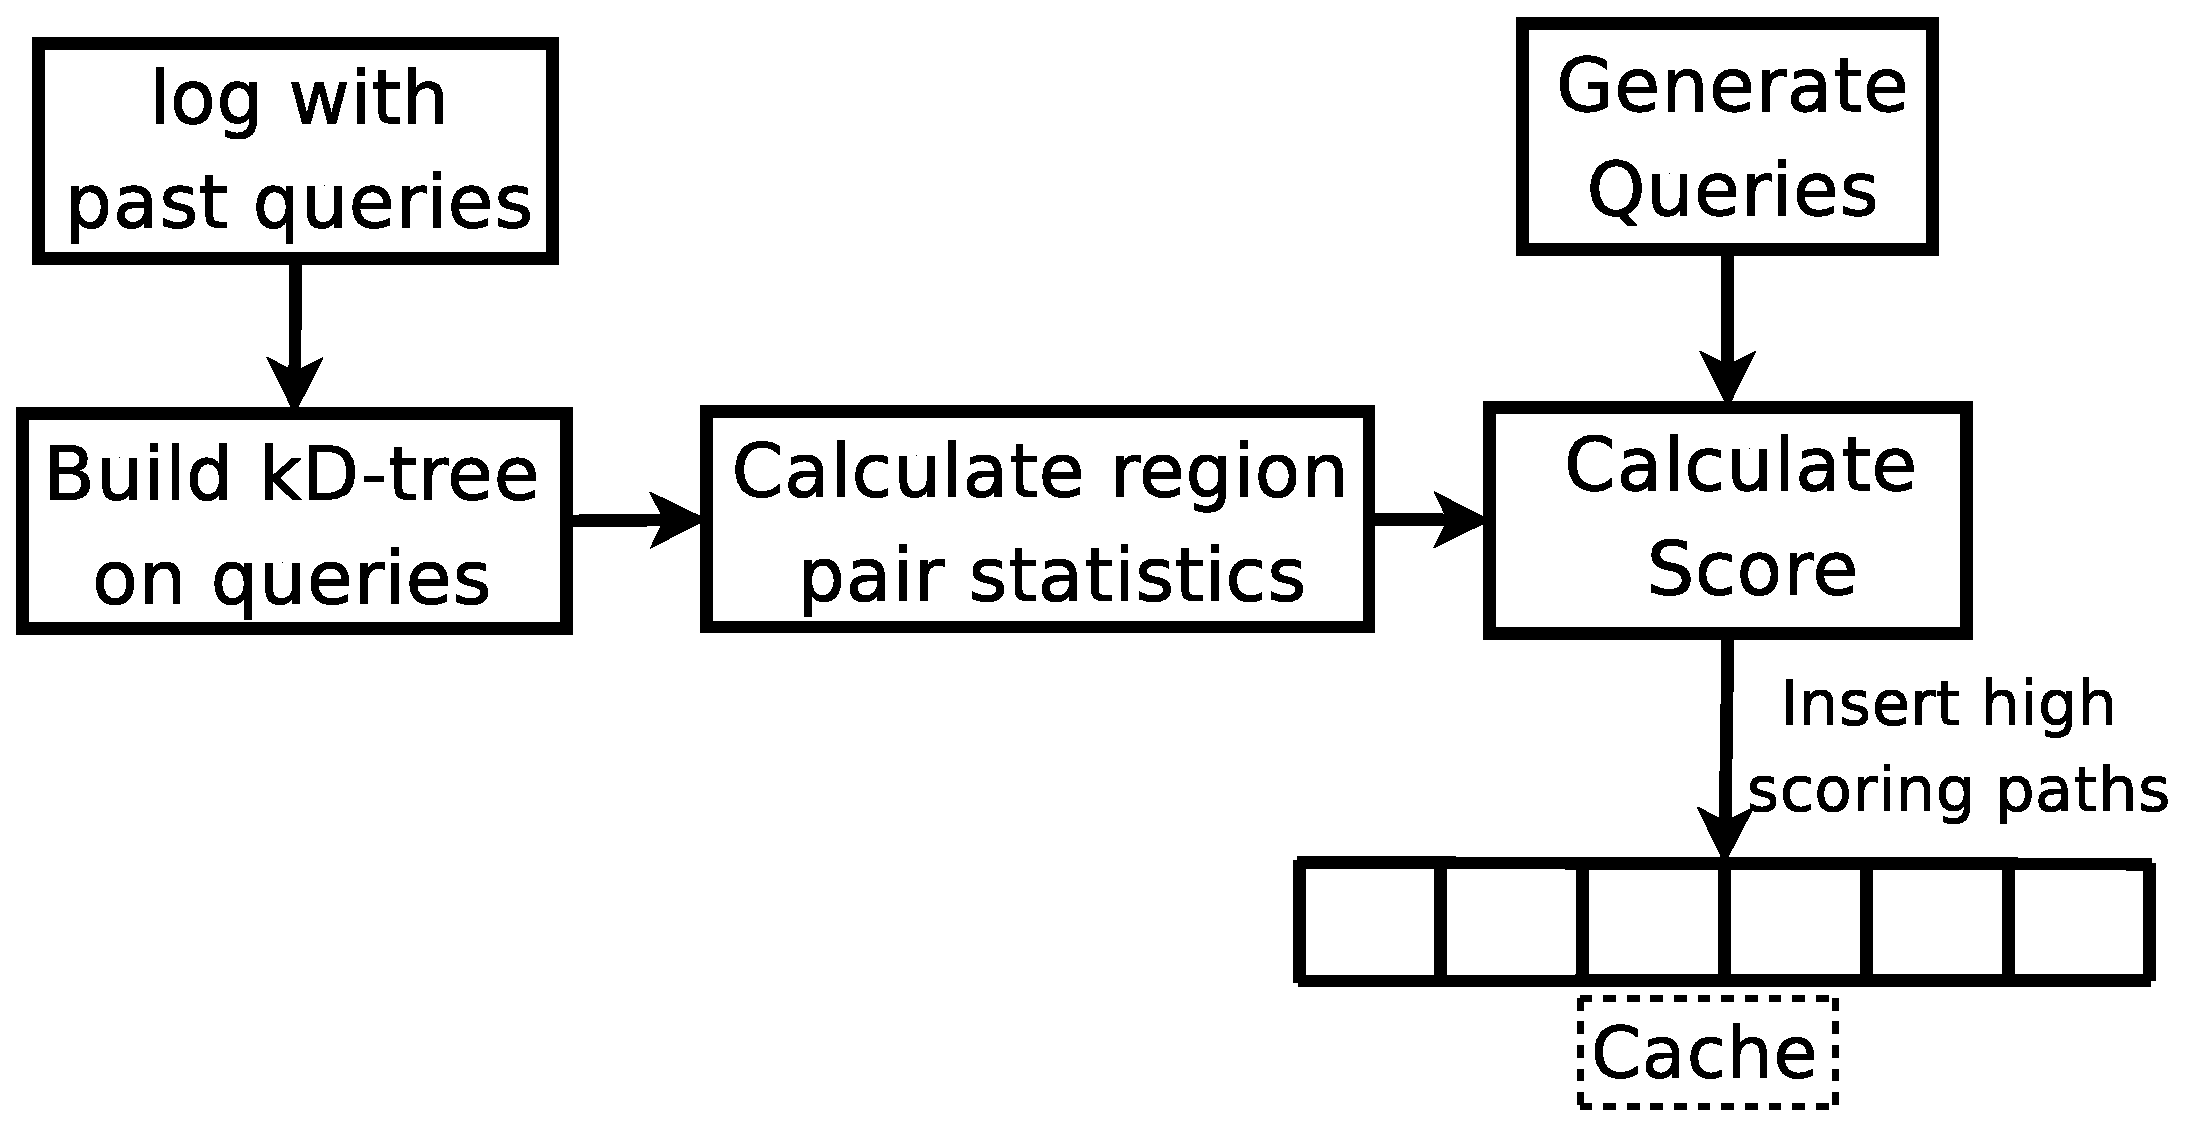
\includegraphics[width=0.5\textwidth]{figures/fillcache}
        \caption{Insertion of buffer elements in offline phase.}
  \label{fig:routequery}
\end{figure}



\begin{table}
\begin{tabular*}{\columnwidth}{|l||p{0.77\columnwidth}|}
\hline
\bf Symbol          & \bf Meaning \\\hline
\spath          & Shortest Path \\\hline
LRU             & Least Recently Used \\\hline
FIFO            & First In First Out \\\hline
OSC             & Optimal Substructure Cache \\\hline
\acs{SPS}       & \acl{SPS} \\\hline
\end{tabular*}
\caption{Table of symbols and notation}
\label{tab:symbols}
\end{table}





\section{..}

\subsection{helping text}
\begin{enumerate}
\item Introduce the problem setting in more detail than in the introduction and formally define the problem and what exactly we aim to solve in this paper.\\
\item show where exactly the proposed cache is located in an online \spath service providers system.
\item State goal 1(a) and 2(b)
	\begin{enumerate}
	\item Reduce the time spent executing the \spath algorithm. - The \spath algorithm is usually the single most CPU expensive task at a \spath service provider.
	\item Reduce the time spent on overhead. - Introducing a cache will also add some overhead, this overhead not desirable and should  be minimized.
	\end{enumerate}
\item Introduce the overall setting which our solution work in and give a table of notation for reader reference.
\end{enumerate}

% 
% Our "cache" is a static cache.
% It sounds better if use the term "buffer" rather than "cache".
% 
% 
% For the paper, you can start writing the "problem setting".
% 
% Try to think all necessary issues for clarifying the problem setting.
% 
% E.g., why do we need a "buffer" ?
%      where is the "buffer" located ?